\documentclass[14pt]{extbook}
\usepackage{multicol, enumerate, enumitem, hyperref, color, soul, setspace, parskip, fancyhdr} %General Packages
\usepackage{amssymb, amsthm, amsmath, latexsym, units, mathtools} %Math Packages
\everymath{\displaystyle} %All math in Display Style
% Packages with additional options
\usepackage[headsep=0.5cm,headheight=12pt, left=1 in,right= 1 in,top= 1 in,bottom= 1 in]{geometry}
\usepackage[usenames,dvipsnames]{xcolor}
\usepackage{dashrule}  % Package to use the command below to create lines between items
\newcommand{\litem}[1]{\item#1\hspace*{-1cm}\rule{\textwidth}{0.4pt}}
\pagestyle{fancy}
\lhead{Progress Quiz 7}
\chead{}
\rhead{Version B}
\lfoot{4173-5738}
\cfoot{}
\rfoot{Spring 2021}
\begin{document}

\begin{enumerate}
\litem{
Solve the quadratic equation below. Then, choose the intervals that the solutions $x_1$ and $x_2$ belong to, with $x_1 \leq x_2$.\[ 10x^{2} +57 x + 54 = 0 \]\begin{enumerate}[label=\Alph*.]
\item \( x_1 \in [-46.2, -42] \text{ and } x_2 \in [-12.33, -11.78] \)
\item \( x_1 \in [-10.5, -7.8] \text{ and } x_2 \in [-0.69, -0.43] \)
\item \( x_1 \in [-14.1, -12.5] \text{ and } x_2 \in [-0.49, -0.17] \)
\item \( x_1 \in [-2.7, 0] \text{ and } x_2 \in [-2.6, -2.15] \)
\item \( x_1 \in [-4.6, -4.1] \text{ and } x_2 \in [-1.37, -1.19] \)

\end{enumerate} }
\litem{
Graph the equation below.\[ f(x) = (x+1)^2 - 20 \]\begin{enumerate}[label=\Alph*.]
\begin{multicols}{2}\item 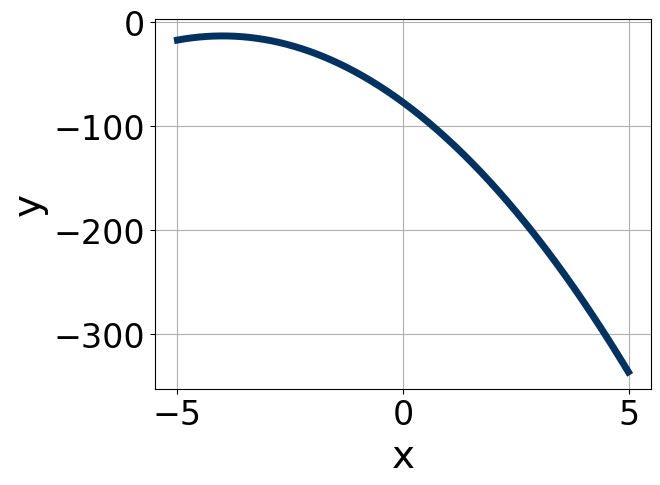
\includegraphics[width = 0.3\textwidth]{../Figures/quadraticEquationToGraphCopyAB.png}\item 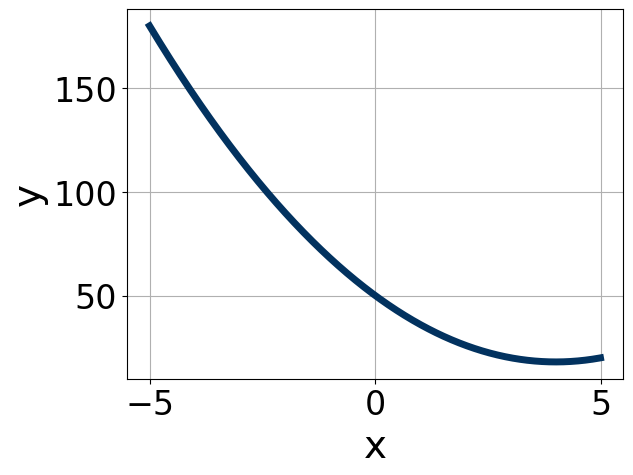
\includegraphics[width = 0.3\textwidth]{../Figures/quadraticEquationToGraphCopyBB.png}\item 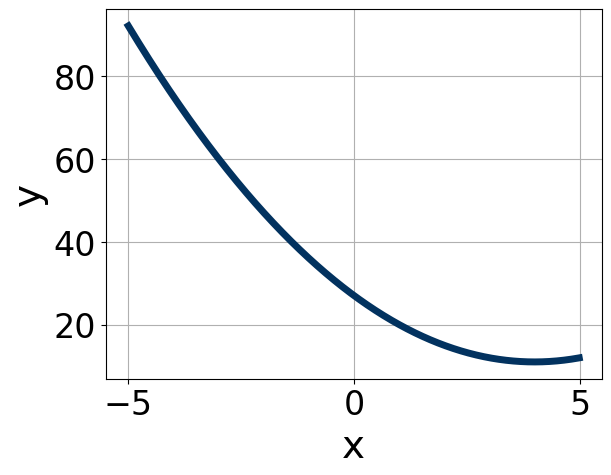
\includegraphics[width = 0.3\textwidth]{../Figures/quadraticEquationToGraphCopyCB.png}\item 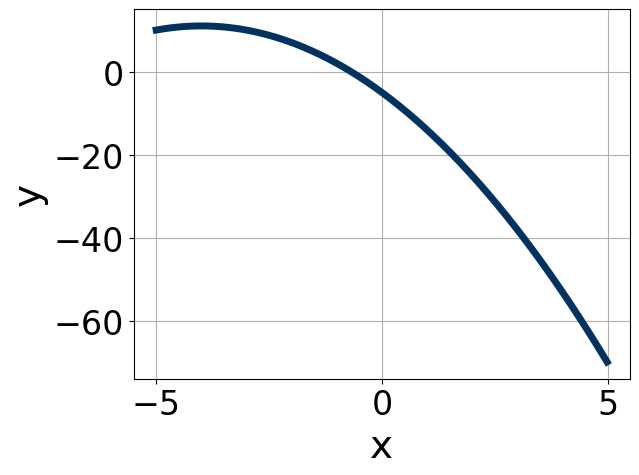
\includegraphics[width = 0.3\textwidth]{../Figures/quadraticEquationToGraphCopyDB.png}\end{multicols}\item None of the above.
\end{enumerate} }
\litem{
Solve the quadratic equation below. Then, choose the intervals that the solutions belong to, with $x_1 \leq x_2$ (if they exist).\[ -14x^{2} +12 x + 8 = 0 \]\begin{enumerate}[label=\Alph*.]
\item \( x_1 \in [-1.7, -0.5] \text{ and } x_2 \in [-1.1, 0.5] \)
\item \( x_1 \in [-18.5, -16.8] \text{ and } x_2 \in [5.9, 6.8] \)
\item \( x_1 \in [-0.9, -0.1] \text{ and } x_2 \in [1.1, 1.8] \)
\item \( x_1 \in [-25.3, -23.3] \text{ and } x_2 \in [24.5, 27] \)
\item \( \text{There are no Real solutions.} \)

\end{enumerate} }
\litem{
Solve the quadratic equation below. Then, choose the intervals that the solutions $x_1$ and $x_2$ belong to, with $x_1 \leq x_2$.\[ 15x^{2} -8 x -16 = 0 \]\begin{enumerate}[label=\Alph*.]
\item \( x_1 \in [-5.09, -3.54] \text{ and } x_2 \in [0.07, 0.36] \)
\item \( x_1 \in [-0.46, -0.16] \text{ and } x_2 \in [2.57, 2.78] \)
\item \( x_1 \in [-1.62, -0.85] \text{ and } x_2 \in [0.61, 0.8] \)
\item \( x_1 \in [-12.62, -9.94] \text{ and } x_2 \in [19.51, 20.25] \)
\item \( x_1 \in [-1.26, -0.63] \text{ and } x_2 \in [1.09, 1.69] \)

\end{enumerate} }
\litem{
Graph the equation below.\[ f(x) = (x+2)^2 - 14 \]\begin{enumerate}[label=\Alph*.]
\begin{multicols}{2}\item 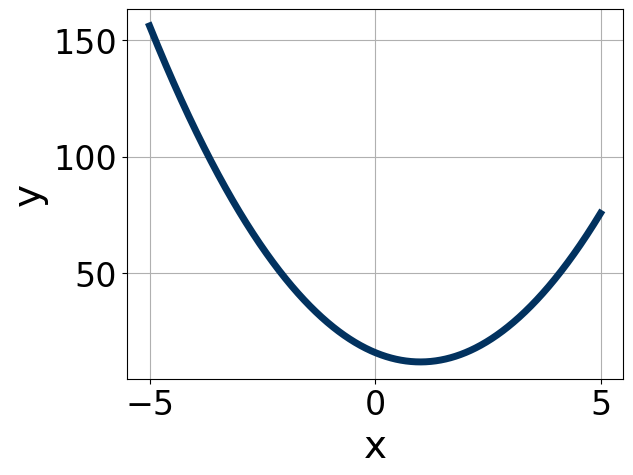
\includegraphics[width = 0.3\textwidth]{../Figures/quadraticEquationToGraphAB.png}\item 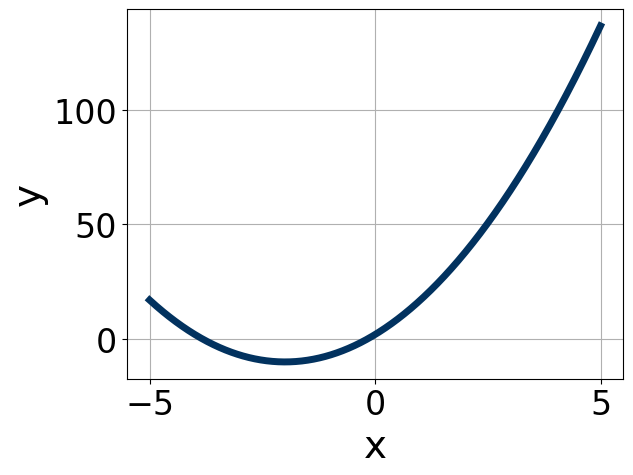
\includegraphics[width = 0.3\textwidth]{../Figures/quadraticEquationToGraphBB.png}\item 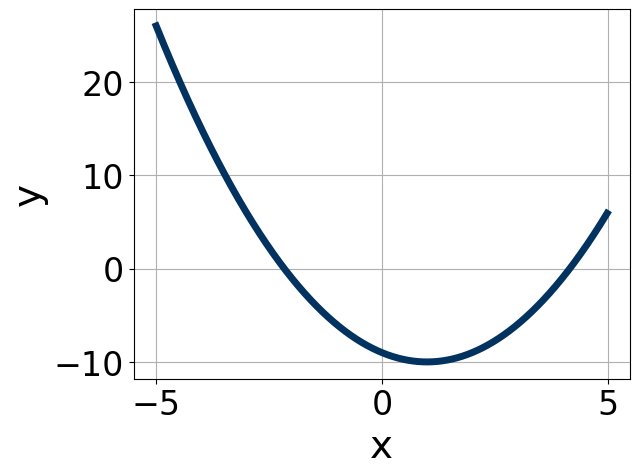
\includegraphics[width = 0.3\textwidth]{../Figures/quadraticEquationToGraphCB.png}\item 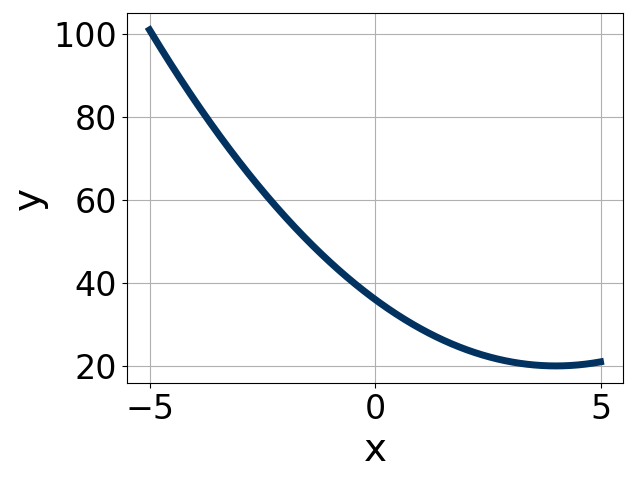
\includegraphics[width = 0.3\textwidth]{../Figures/quadraticEquationToGraphDB.png}\end{multicols}\item None of the above.
\end{enumerate} }
\litem{
Write the equation of the graph presented below in the form $f(x)=ax^2+bx+c$, assuming  $a=1$ or $a=-1$. Then, choose the intervals that $a, b,$ and $c$ belong to.
\begin{center}
    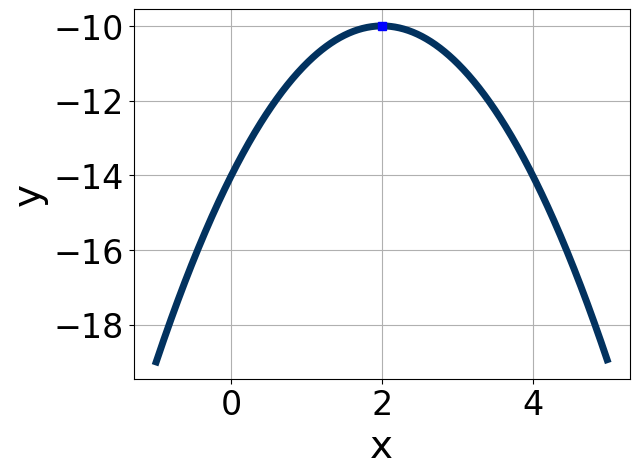
\includegraphics[width=0.5\textwidth]{../Figures/quadraticGraphToEquationB.png}
\end{center}
\begin{enumerate}[label=\Alph*.]
\item \( a \in [-2.3, -0.2], \hspace*{5mm} b \in [7, 11], \text{ and } \hspace*{5mm} c \in [-30, -24] \)
\item \( a \in [-0.6, 2.5], \hspace*{5mm} b \in [7, 11], \text{ and } \hspace*{5mm} c \in [26, 28] \)
\item \( a \in [-2.3, -0.2], \hspace*{5mm} b \in [-9, -6], \text{ and } \hspace*{5mm} c \in [-7, -3] \)
\item \( a \in [-2.3, -0.2], \hspace*{5mm} b \in [7, 11], \text{ and } \hspace*{5mm} c \in [-7, -3] \)
\item \( a \in [-0.6, 2.5], \hspace*{5mm} b \in [-9, -6], \text{ and } \hspace*{5mm} c \in [26, 28] \)

\end{enumerate} }
\litem{
Factor the quadratic below. Then, choose the intervals that contain the constants in the form $(ax+b)(cx+d); b \leq d.$\[ 36x^{2} +60 x + 25 \]\begin{enumerate}[label=\Alph*.]
\item \( a \in [4, 7.5], \hspace*{5mm} b \in [-1, 10], \hspace*{5mm} c \in [3.7, 8.2], \text{ and } \hspace*{5mm} d \in [5, 6] \)
\item \( a \in [10, 13.3], \hspace*{5mm} b \in [-1, 10], \hspace*{5mm} c \in [1.3, 3.4], \text{ and } \hspace*{5mm} d \in [5, 6] \)
\item \( a \in [1.8, 3.2], \hspace*{5mm} b \in [-1, 10], \hspace*{5mm} c \in [8.4, 12.3], \text{ and } \hspace*{5mm} d \in [5, 6] \)
\item \( a \in [0.7, 2.8], \hspace*{5mm} b \in [29, 37], \hspace*{5mm} c \in [-0.5, 1.6], \text{ and } \hspace*{5mm} d \in [29, 34] \)
\item \( \text{None of the above.} \)

\end{enumerate} }
\litem{
Factor the quadratic below. Then, choose the intervals that contain the constants in the form $(ax+b)(cx+d); b \leq d.$\[ 24x^{2} -10 x -25 \]\begin{enumerate}[label=\Alph*.]
\item \( a \in [3.69, 5.18], \hspace*{5mm} b \in [-9, -3], \hspace*{5mm} c \in [4.6, 7.5], \text{ and } \hspace*{5mm} d \in [2, 14] \)
\item \( a \in [1.01, 2.09], \hspace*{5mm} b \in [-9, -3], \hspace*{5mm} c \in [11.2, 15.8], \text{ and } \hspace*{5mm} d \in [2, 14] \)
\item \( a \in [7.86, 8.2], \hspace*{5mm} b \in [-9, -3], \hspace*{5mm} c \in [2.3, 3.7], \text{ and } \hspace*{5mm} d \in [2, 14] \)
\item \( a \in [0.89, 1.78], \hspace*{5mm} b \in [-33, -27], \hspace*{5mm} c \in [-1.9, 2.5], \text{ and } \hspace*{5mm} d \in [20, 25] \)
\item \( \text{None of the above.} \)

\end{enumerate} }
\litem{
Write the equation of the graph presented below in the form $f(x)=ax^2+bx+c$, assuming  $a=1$ or $a=-1$. Then, choose the intervals that $a, b,$ and $c$ belong to.
\begin{center}
    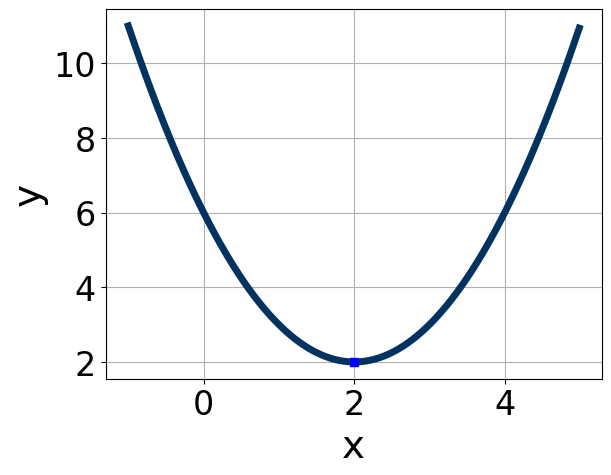
\includegraphics[width=0.5\textwidth]{../Figures/quadraticGraphToEquationCopyB.png}
\end{center}
\begin{enumerate}[label=\Alph*.]
\item \( a \in [0.7, 3.1], \hspace*{5mm} b \in [-6, 0], \text{ and } \hspace*{5mm} c \in [-2, 3] \)
\item \( a \in [-1.5, -0.3], \hspace*{5mm} b \in [3, 6], \text{ and } \hspace*{5mm} c \in [-2, 3] \)
\item \( a \in [-1.5, -0.3], \hspace*{5mm} b \in [-6, 0], \text{ and } \hspace*{5mm} c \in [-8, -6] \)
\item \( a \in [0.7, 3.1], \hspace*{5mm} b \in [3, 6], \text{ and } \hspace*{5mm} c \in [-2, 3] \)
\item \( a \in [-1.5, -0.3], \hspace*{5mm} b \in [3, 6], \text{ and } \hspace*{5mm} c \in [-8, -6] \)

\end{enumerate} }
\litem{
Solve the quadratic equation below. Then, choose the intervals that the solutions belong to, with $x_1 \leq x_2$ (if they exist).\[ 14x^{2} -9 x -2 = 0 \]\begin{enumerate}[label=\Alph*.]
\item \( x_1 \in [-1.24, -0.76] \text{ and } x_2 \in [-0.06, 0.78] \)
\item \( x_1 \in [-0.49, 0.03] \text{ and } x_2 \in [0.81, 1.43] \)
\item \( x_1 \in [-14.04, -12.76] \text{ and } x_2 \in [13.1, 14.86] \)
\item \( x_1 \in [-3.19, -2.28] \text{ and } x_2 \in [10.49, 12.03] \)
\item \( \text{There are no Real solutions.} \)

\end{enumerate} }
\end{enumerate}

\end{document}